\documentclass[11pt,a4paper]{article}


\setlength{\topmargin}{-55pt}%
\setlength{\oddsidemargin}{-20pt}%
\setlength{\textwidth}{490pt}%
\setlength{\textheight}{700pt}%
\setlength{\headsep}{20pt}%
\setlength{\headheight}{14pt}

\usepackage[utf8]{inputenc} % accents 8 bits dans le fichier
\usepackage[T1]{fontenc}      % accents codés dans la fonte
\usepackage[french]{babel}
\usepackage{amsmath,amssymb}
\usepackage{graphicx}
\usepackage{fancyhdr}
\usepackage{booktabs}
\usepackage{color, colortbl}
\usepackage{appendix}
\usepackage{pgfplots}
\usepackage[hidelinks]{hyperref}
\usepackage{siunitx}
\usepackage{subcaption}

\pgfplotsset{compat=1.3}

\pgfplotsset{
    discard if not/.style 2 args={
        x filter/.code={
            \edef\tempa{\thisrow{#1}}
            \edef\tempb{#2}
            \ifx\tempa\tempb
            \else
                \def\pgfmathresult{inf}
            \fi
        }
    }
}

\addto\captionsfrench{% Replace "english" with the language you use
  \renewcommand{\contentsname}%
    {Table des matières}
}

\DecimalMathComma

\lhead{}      %en-tête
\chead{AOC : Application MiniMD}%
\rhead{}%
\lfoot{\tiny{Pierre GRANGER \& Matthias BEAUPERE}}
\cfoot{}%
\rfoot{\thepage}%
\renewcommand{\headrulewidth}{0.5pt}
\renewcommand{\footrulewidth}{0.5pt}
\pagestyle{fancy}

\newcommand{\HRule}{\rule{\linewidth}{0.5mm}}
\newcommand{\norm}[1]{\left\lVert#1\right\rVert}

\definecolor{green}{rgb}{0.2,0.8,0.2}

\begin{document}
\begin{center}

	{\LARGE\centering Projet d'AOC :\\ Application de test MiniMD}\\[1cm]

	{ Matthias \bsc{Beaupère}, Pierre \bsc{Granger}}\\[0.5cm]
	{Rapport AOC - CHPS - \today}\\[2cm]
\end{center}

\tableofcontents
\newpage

\section{Dynamique moléculaire}
	La dynamique moléculaire est un domaine de la simulation numérique qui s'intéresse à l'évolution des systèmes d'atomes dans le temps et qui cherche à en déduire les configurations énergétiques les plus favorables. Cela peut par exemple permettre d'étudier le repliement des protéines afin d'en déduire des connaissances dans le domaine de la biologie.
	Une simulation de dynamique moléculaire est un processus itératif. A chaque nouveau pas de temps, on calcule les interactions entre chaque paire d'atomes afin d'en déduire les forces qui s'appliquent sur chaque atome puis le mouvement de ces derniers durant le pas de temps considéré.

\section{Présentation de l'application}
	L'application sur laquelle nous avons travaillé est MiniMD. Cette application de simulation en dynamique moléculaire est écrite en C++ et est parallèle. Son objectif est de pouvoir tester l'efficacité des nouvelles architectures parallèles dans l'exécution de codes de simulation de dynamique moléculaire. Dans cet objectif, cette mini-application a été conçue afin d'être simple et légère ainsi que facilement adaptable sur de nouvelles architectures matérielles. Les algorithmes de base utilisés dans ce code suivent les algorithmes d'un code de dynamique moléculaire de production bien plus important, LAMMPS.

	L'application est écrite en C++ et comporte moins de 5000 lignes de code. Elle permet d'effectuer des simulations de dynamique moléculaire avec des potentiels de Lennard-Jones ou des modèles EAM (Emnbedded Atom Model) uniquement. La parallélisation des calculs est effectuée via une décomposition spatiale du domaine d'étude : chaque processeur du cluster effectue ses calculs sur une partie du domaine de simulation. Le code est sensé passer correctement à l'échelle  sur une architecture parallèle. L'application peut fonctionner avec plusieurs librairies de parallélisation proposant des types de parallélisme différents : MPI, OpenMP, OpenCL, Kokkos, OpenACC, \ldots Dans ce rapport, seule l'implémentation utilisant MPI pour le parallélisme en mémoire distribuée et OpenMP pour le parallélisme en mémoire partagée sera étudiée.

	Comme dans des codes de simulations plus complexes, miniMD permet à l'utilisateur de spécifier de nombreux paramètres du problèmes à étudier : la taille du problème, la température, la densité atomique, la durée des pas de temps, le nombre de pas de temps à simuler et la distance de coupure à utiliser pour l'interaction considérée. Néanmoins, seuls deux types d'interactions sont disponibles (Lennard-Jones et EAM). En effet, les interactions électrostatiques à longue distance ainsi que les champs de force moléculaires ne peuvent pas être simulés avec cette application. L'ajout de telles fonctionnalités n'aurait fait que compliquer le code alors qu'elles ne sont pas nécessaires afin d'effectuer des tests avec de la dynamique moléculaire basique. Avec ses fonctionnalités limités, miniMD permet à des personnes n'étant pas des experts de la dynamique moléculaire d'effectuer des tests de performance à l'aide de ce code.

	Afin d'optimiser les calculs de forces ressenties par chaque atome, miniMD utilise des listes d'atomes voisins tout comme la majorité des codes de dynamique moléculaire actuels. Cette technique a l'inconvénient d'utiliser plus de mémoire, c'est à dire environ 1GB pour 500000 atomes simulés.

	Dans sa dernière version, miniMD offre la possibilité de simulés des atomes de nature différente ce qui n'était pas le cas dans sa première version. Cette fonctionnalité, qui permet de mieux modéliser le comportement d'un code de dynamique moléculaire de production, dégrade les performances par rapport à la version initiale. En effet, l'introduction de plusieurs types d'atomes ajoute des indirections au sein du code ce qui le ralentit et diminue les possibilités de vectorisation de ce dernier.

	\subsection{Compilation de l'application}
		Comme expliqué précédemment, nous compilons la version utilisant MPI et OpenMP. Ses sources peuvent être trouvées dans le sous dossier \textit{ref}. Le code peut alors être simplement compilé en exécutant la commande \textit{make openmpi}. Une fois compilé, le programme peut être testé en utilisant la commande \textit{make test}. Les tests réalisés s'appuient sur des comparaisons avec des résultats précalculés et fournis avec le code source du programme.
\section{Bilan de performances}

	\subsection{Cadre d'expérimentation}
		
		\subsubsection{Matériel d'expérimentation}

			Le programme miniMD est compilé puis exécuté sur un PC de bureau sous Linux Mint ayant 8 Go de mémoire vive et un processeur Intel I3 2.8 GHz de première génération. Ce processeur a une micro-architecture de type Nehalem qui à une vectorisation SSE 4.2. Une telle architecture permet d'effectuer des opérations sur des blocs de 128 bits.

		\subsubsection{Compilation}

			Le programme est compilé avec \texttt{gcc} version 5.4 ainsi que les options \texttt{-Ofast} activant les optimisations du compilateur et \texttt{--funroll-loops} qui optimise le déroulement des boucles. L'option \texttt{-g} est également présente pour pouvoir effectuer le profiling.

		\subsubsection{Exécution et profiling}

			La mini-app permet un paramétrage fin du problème physique sous-jacent. Nous avons ainsi pu dimensionner le problème pour avoir un temps d'exécution d'environ 40 secondes sur la machine présentée plus haut, ce qui conduit à la génération d'un million d'atomes.

			La mini-app est exécutée à travers un profiler, ce qui permet de générer un bilan de performances pour un exécution de l'application. Nous avons choisi le profiler Maqao qui permet de visualiser les points chauds et donne des conseils d'optimisation utiliser pleinement les performances de la micro-architecture. Avec Maqao, on utilise le module \texttt{oneview} qui appelle les différents modules d'analyse de l'exécution puis met en page les résultats dans une page web.

	\subsection{Résultats}

		\subsubsection{Métriques globales}

			\begin{figure}[h!]
				\begin{center}
					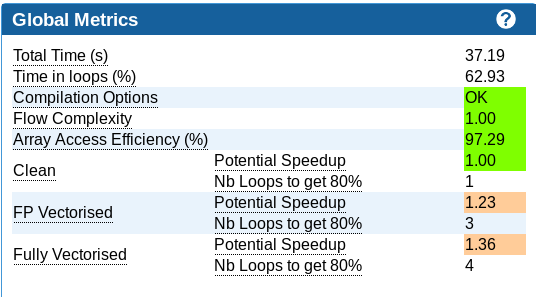
\includegraphics{images/maqao_global_metrics.png}
					\caption{Métriques global obtenu avec Maqao pour 4 threads}
					\label{global_maqao}
				\end{center}
			\end{figure}

			La figure \ref{global_maqao} donne les résultats obtenus pour un run avec Maqao avec 4 threads sur la machine présentée ci-dessus. On observe que les résultats sont particulièrement bon. Tout d'abord \textit{Flow Complexity} est au minimum, c'est à dire que le flot de contrôle est prévisible et donc que les prédicateurs de branchement sont très efficaces. Ensuite \textit{Array Access Efficiency} est à 97\% ce qui témoigne d'un très bon accès mémoire, notamment grâce à des accès contigus qui génèrent peu de défaut de cache. Maqao nous dit même clairement qu'aucune optimisation n'est vraiment envisageable en séquentielle sans prendre en compte la capacité à vectoriser.

			Du côté de la vectorisation, le résultat est plus mitigé. On sait que l'unité de calcul utilisé peu vectoriser 128 bits en parallèle, c'est ça dire 4 \texttt{float} ou 2 \texttt{doubles}, ce qui conduit dans le cas théorique à une accélération maximum de 4 pour des opération sur des \texttt{float} et 2 pour des opérations sur les \texttt{doubles}. D'après les métrique de Maqao, une accélération entre 1 et 2 est possible grâce à la vectorisation.

		\subsubsection{Points chauds}

			\begin{figure}[h!]
				\begin{center}
					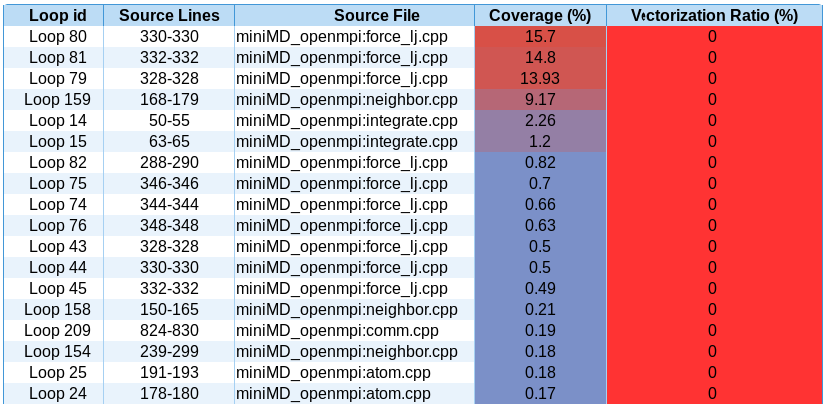
\includegraphics[width=500px]{images/maqao_loops.png}
					\caption{Statistiques des boucles obtenu avec Maqao pour 4 threads}
					\label{loop_maqao}
				\end{center}
			\end{figure}

			La figure \ref{loop_maqao} donne la part du temps d'exécution global que représente chaque boucle du programme. Un première résultat intéressant est qu'aucune boucle n'a été vectorisé. Cela constitue une bonne piste pour l'optimisation. Par ailleurs, on voit que les 62\% du temps d'exécution liés au boucle sont essentiellement répartis, environ 42\% sur les 62\%, sur trois boucles qui ne font qu'une ligne chacune. En regardant dans le détail la localisation des trois lignes, on se rend compte qu'elle sont côte-à-côte.

			La figure \ref{code:hotspot} donne les lignes correspondantes. On remarque la présence de \verb!#pragma omp atomic! qui permet d'empêcher les \textit{race condition} entre le threads pour la mise à jour des données. Ces 

			\begin{figure}[h!]
				\caption{Extrait de code correspondant au point chaud}
				\label{code:hotspot}
				\begin{verbatim}
					  #pragma omp atomic
					  f[j * PAD + 0] -= delx * force;
					  #pragma omp atomic
					  f[j * PAD + 1] -= dely * force;
					  #pragma omp atomic
					  f[j * PAD + 2] -= delz * force;
				\end{verbatim}
			\end{figure}




\section{Résultats MPI et OMP}
	\begin{figure}
		\centering
		\begin{tikzpicture}[scale=1.5]
			\begin{axis}[minor tick num=1,
				xlabel=Nombre total de threads,
				ylabel=Temps d'exécution (\si{\second}),
				ymin=0,
				ymax=66]
			\addplot [green, mark=*, discard if not={MPI}{1}] table [x={OMP}, y={t}] {data.res};
			\addplot [blue, mark=*, discard if not={MPI}{2}] table [x expr=\thisrowno{1}*2, y={t}] {data.res};
			\addplot [red, mark=*, discard if not={MPI}{4}] table [x expr=\thisrowno{1}*4, y={t}] {data.res};
			\draw [dashed] (axis cs:9, \pgfkeysvalueof{/pgfplots/ymin}) -- (axis cs:9, \pgfkeysvalueof{/pgfplots/ymax});
			\legend{MPI = 1, MPI = 2, MPI = 4}
			\addlegendimage{dashed}
			\addlegendentry{Hyperthreading}
			\end{axis}
		\end{tikzpicture}
		\caption{Evolution du temps d'exécution en fonction du nombre de processus MPI et du nombre total de threads.\label{fig:tvsparallel}}
	\end{figure}
\end{document}
